\subsection{Unit Tests and Cross Checks}
\label{sec:unit_tests_and_cross_checks}

There are several techniques to ensure that the propagation algorithm
produces results that meet the expectations. First, \clsim itself
implements a number of tests that run in each simulation and check
computational quantities for consistency. \cite{clsimsource}

Secondly, one can define scenarios with known quantities for single
photons and check externally whether the algorithm produces the expected
results for those single photons. This is done with \textit{unit tests}
and is presented in section \ref{sec:unit_tests}.

Thirdly, checks for a sample of photons can be devised where all photons
should behave the same way, for example all photons should be absorbed
by a medium that is configured for instant absorption. This check is
presented in section \ref{sec:instant_absorption_tests}.

Finally, a sample of propagated photons can be examined regarding their
statistical properties, for example the sample's distributions of
quantities like arrival time and path length. These tests are presented
in sections \ref{sec:arrival_time} to \ref{sec:cross_check_71}.

\subsubsection{Unit Tests With Single
Photons}\label{unit-tests-with-single-photons}

\label{sec:unit_tests}

In order to verify that individual components (``units'') of the
implementation produce results as expected, unit tests were implemented
for the algorithm that calculates intersections as well as for the
hole-ice-correction algorithm.

\docframe{
  \sourceparwithoutframe{The unit tests for the intersection algorithm can be found in the folder \texttt{unit\_tests} on the CD-ROM and at \url{https://github.com/fiedl/clsim/blob/sf/hole-ice-2017/resources/kernels/lib/intersection/intersection_test.c}.}\medskip

  \sourceparwithoutframe{The unit tests for the hole-ice-correction algorithm can be found in the folder \texttt{unit\_tests} on the CD-ROM and at \url{https://github.com/fiedl/clsim/blob/sf/hole-ice-2017/resources/kernels/lib/hole_ice/hole_ice_test.c}.}
}

\paragraph{Task}

The task of unit tests is to test individual components of a software.
In this case, the tests execute separate functions of the new algorithms
with fixed input parameters and check whether the functions return the
expected results, which, in preparation of the test, have been obtained
by other means, either by a separate program, using a separate
programming language, a separate algorithm, or via calculations by hand.

In this study, unit tests define single photons that cross hole-ice
cylinders in a pre-defined way and check whether the intersection
algorithm determines the correct intersection points, whether the 2d-3d
projections are handled correctly, and whether the hole-ice-correction
algorithm determines the expected corrections for the geometric
distances according to the hole-ice parameters provided by the test
scenario. Extreme examples can be designed to produce simple results
that can be calculated by hand and verified by intuition. For example,
for hole-ice cylinders configured for instant absorption, the absorption
point is identical to the intersection point of the photon trajectory
and the cylinder. More complex examples require more involved
calculations by hand or using other software like \noun{Python} scripts
or computer algebra tools for calculating intersections.

\paragraph{Testing Framework}

This study uses the
\noun{gtest}\footnote{Google Test Framework, gtest, \url{https://github.com/google/googletest}}
testing framework. This framework has been chosen due to its good
documentation, wide adoption and slim architecture that made it possible
to use the framework to test individual components of the new source
code without interfering with the rest of the \icesim framework.

\docpar{The introductory documentation of \noun{gtest} can be found at \url{https://github.com/google/googletest/blob/master/googletest/docs/primer.md}.}

\paragraph{Limitations of Unit Tests}

Unit tests are most useful to ensure stability when adjusting,
refactoring or rewriting software components. Even after replacing a
large part of the source code, unit tests can make sure that the
software still produces the same results as before. Tests also allow for
so-called test-driven development where the expected results are
specified first, and then the software is built or changed iteratively
until it produces the expected results. This technique works best when
the components to be tested have small interfaces because the technique
requires the tests to provide all input parameters for the components to
be tested.

Unexpected issues may arise when unit tests are run on another
architecture as the production code. For example, the unit tests used in
this study were insensitive to certain driver issues and numerical
issues\footnote{See section \ref{sec:gpu_technical_issues}.} that did
only occur when running the software on the GPUs of the computing
cluster and did not occur when running the unit tests on the local CPU
of the development machine.

Unit tests are, by design, also insensitive to high-level problems. Each
individual component may produce the results expected from this
component while still issues may arise when components are not tied
together correctly, or because the expectations for an individual
component may be wrong, which becomes apparent only when adopting a
larger perspective rather than the focused perspective on individual
components.

To increase confidence in the new software, therefore, in addition to
unit testing, high-level cross checks need to be performed as described
in the following subsections.

\subsubsection{Instant-Absorption Tests}\label{instant-absorption-tests}

\label{sec:instant_absorption_tests}

A simple high-level test can be performed by starting several photons
towards a cylinder, which is configured for instant absorption. After
propagating the photons using the new media-propagation algorithm and
recording the path of each individual photon, one can verify the results
making sure than no photon position is recorded inside the
instant-absorption cylinder (figure \ref{fig:chiep7Is}). Additionally,
one can visualize the simulation using the \steamshovel event viewer to
verify that no photon enters the instant-absorption cylinder as shown in
figure \ref{fig:moo9Eiqu}.

\sourcepar{The implementation of this cross check can be found in \issue{67}, \issue{47}, and \issue{22}.}

\begin{figure}[htbp]
  \subcaptionbox{Distribution of the distance to the hole-ice center, evaluated for each scattering step.}{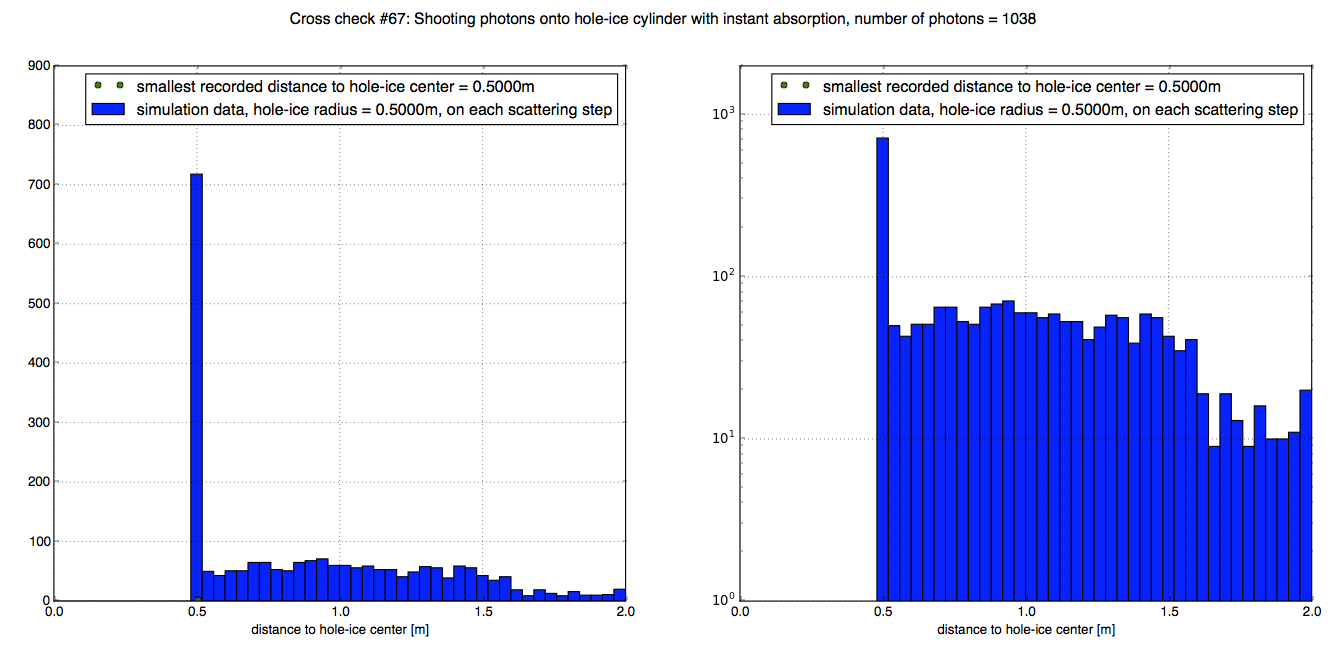
\includegraphics[width=0.32\textwidth, trim={1cm 0 25cm 2cm}, clip]{img/cross-check-67-histogram}}\hfill
  \subcaptionbox{Distance to the next scattering point and distance to hole-ice center for each scattering step.}{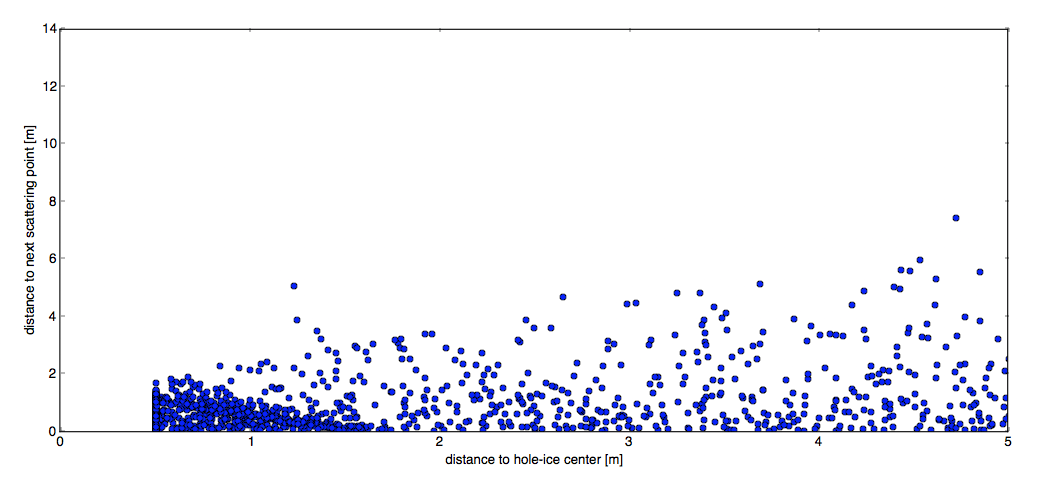
\includegraphics[width=0.65\textwidth, trim={0 0 1cm 0}, clip]{img/cross-check-67-scatter}}
  \caption{Analyzing the simulation of photons propagating towards a hole-ice cylinder configured for instant absorption. No photon can be recorded within the hole-ice cylinder's radius.}
  \label{fig:chiep7Is}
\end{figure}

\begin{figure}[htbp]
  \subcaptionbox{Starting from different positions into the same direction. View from above.}{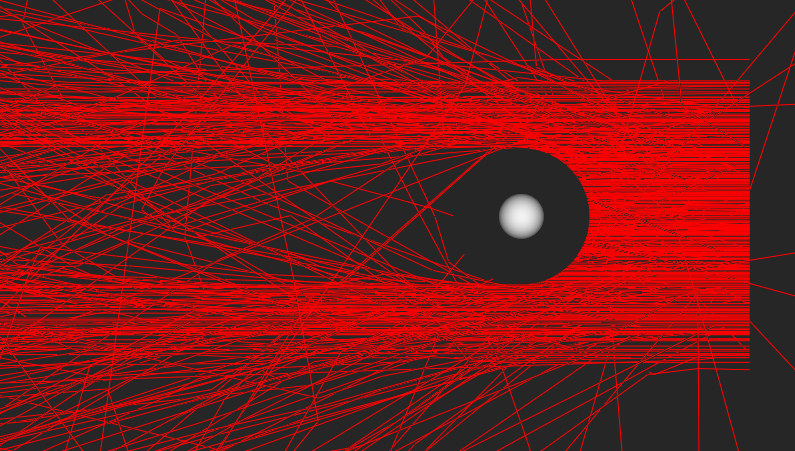
\includegraphics[width=0.49\textwidth]{img/instant-absorption-steamshovel-moo9Eiqu}}\hfill
  \subcaptionbox{Starting from the same position into different directions.}{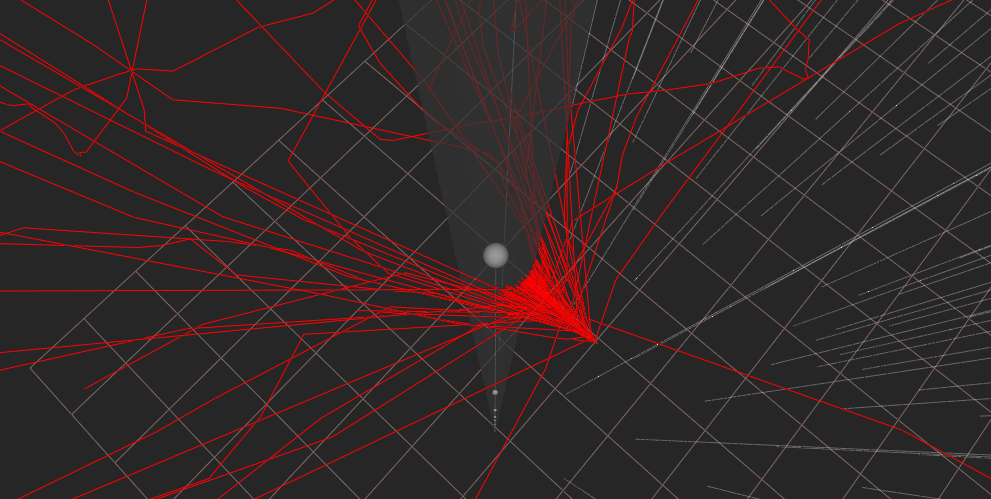
\includegraphics[width=.49\textwidth, trim={0 0 40mm 0}, clip]{img/instant-absorption-steamshovel-Zae4phei}}
  \caption{Visualizing an instant-absorption test using the \steamshovel event viewer. In the simulation, photons are started towards a cylinder configured for instant absorption. If the medium-propagation algorithm works as expected, no photon can get inside the cylinder.}
  \label{fig:moo9Eiqu}
\end{figure}

A related, but more complex scenario is starting photons within two
nested cylinders where the inner cylinder is configured for a short
scattering length and the outer cylinder is configured for instant
absorption (figure \ref{fig:sahmoo8O}).

\begin{figure}[htbp]
  \subcaptionbox{View from above.}{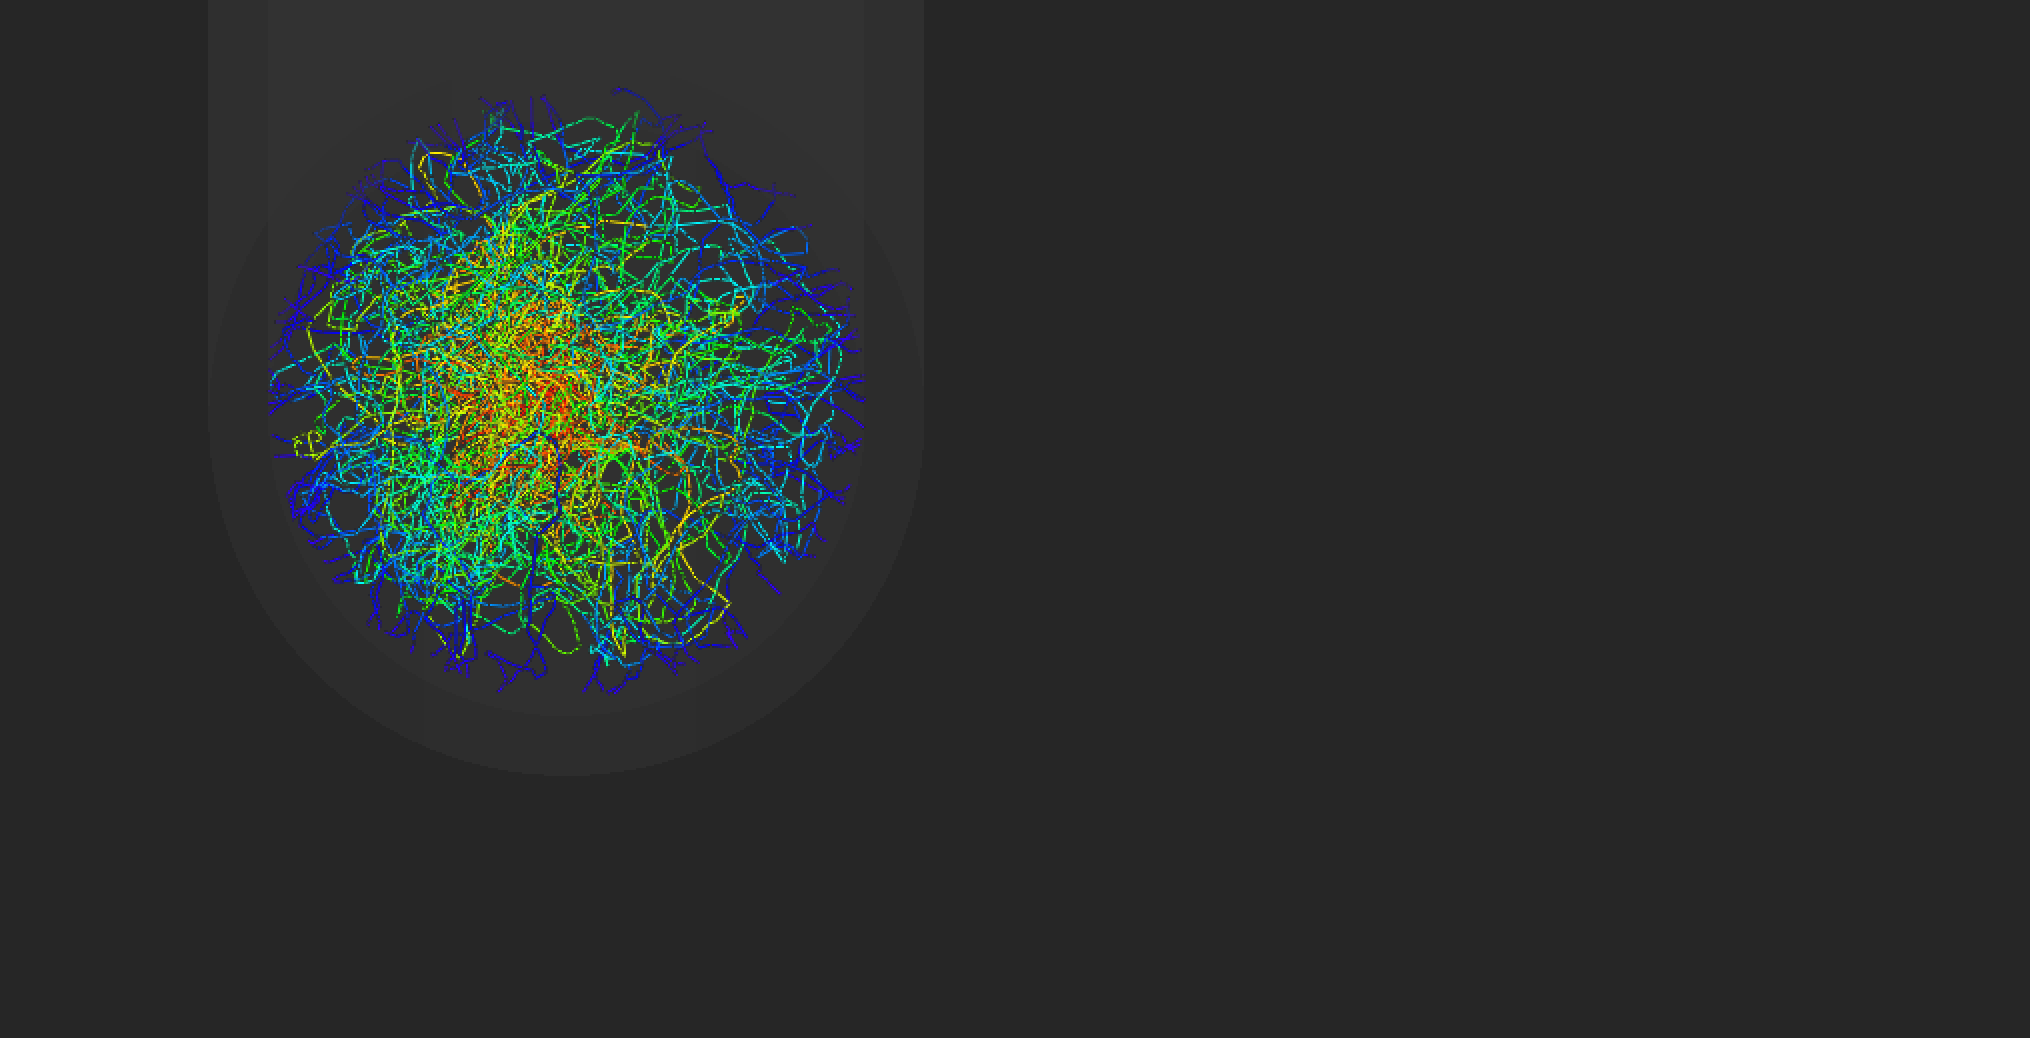
\includegraphics[width=.32\textwidth, trim={0 3cm 16cm 0}, clip]{img/instant-absorption-steamshovel-sahmoo8O-above}}\hfill
  \subcaptionbox{View from the side.}{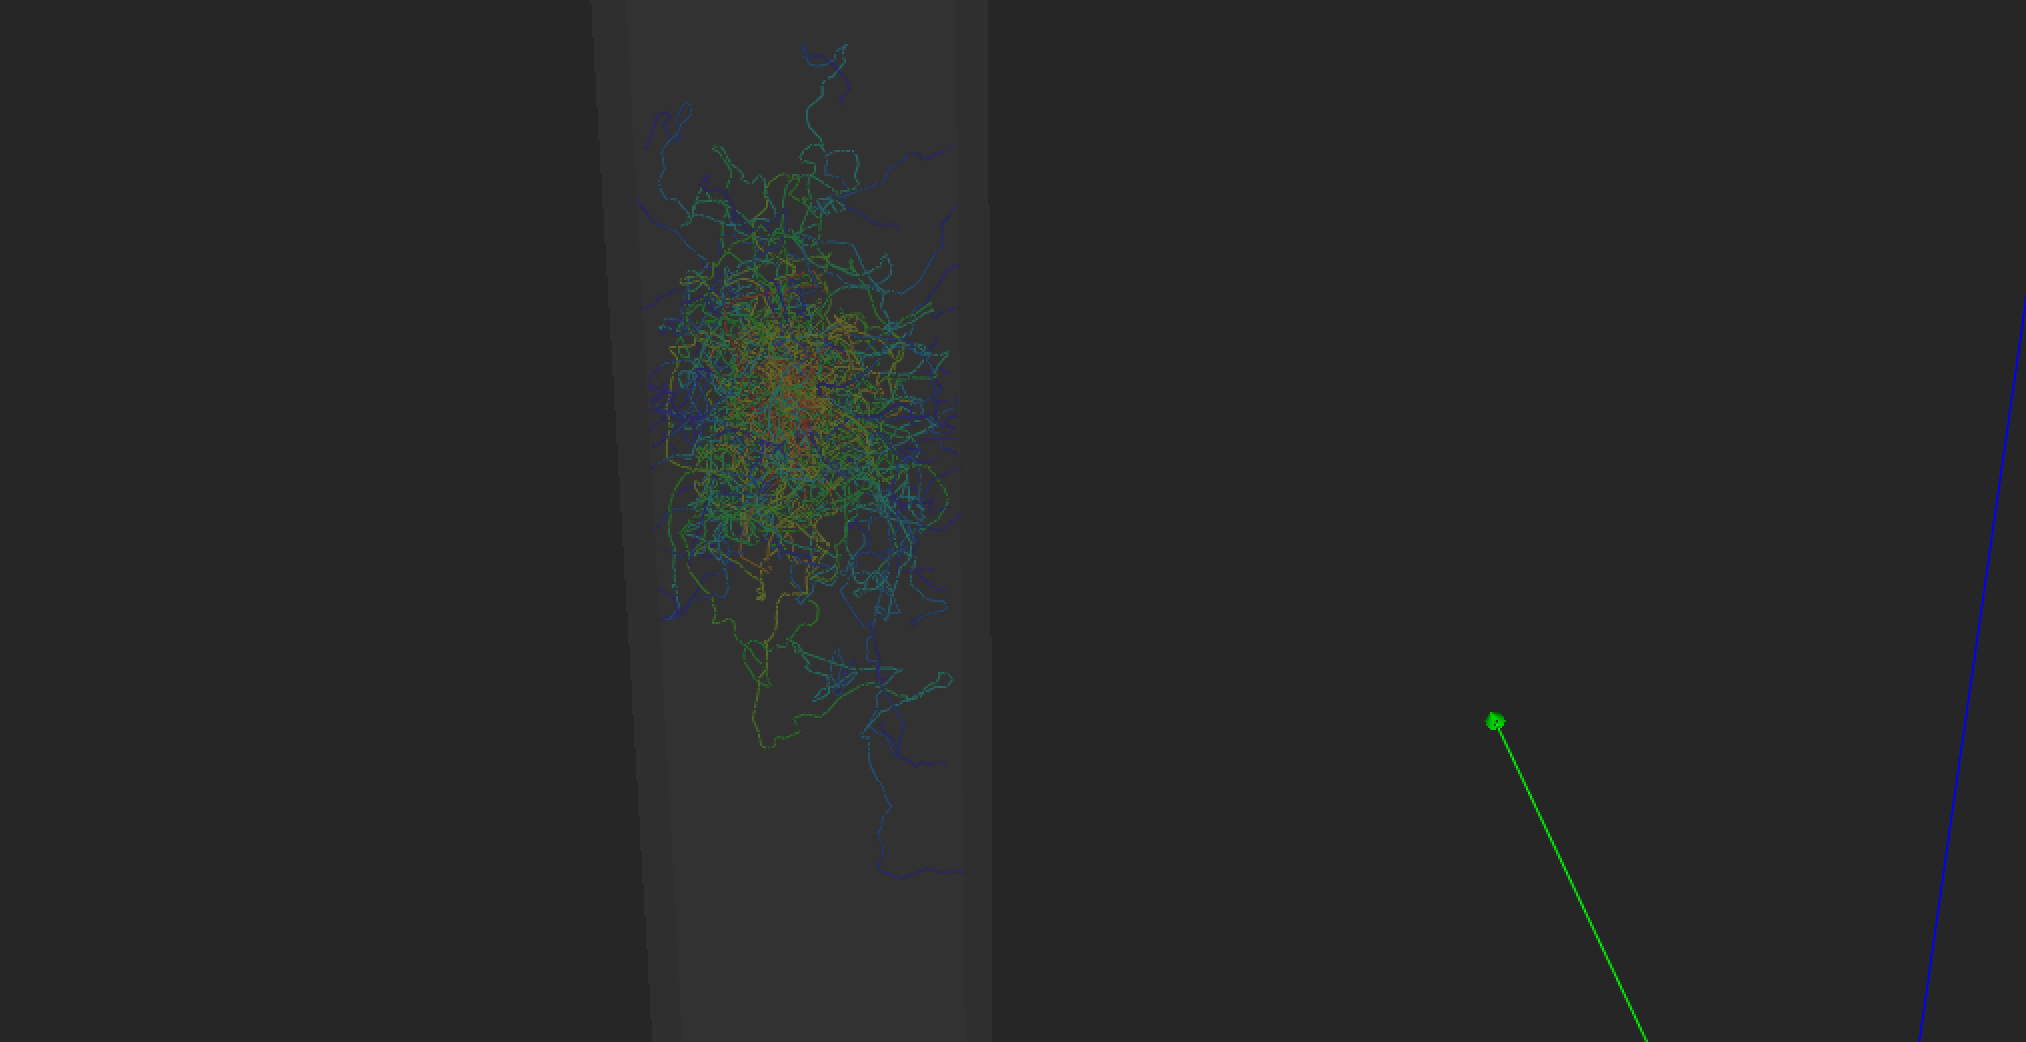
\includegraphics[width=.32\textwidth, trim={6cm 4cm 13cm 1.5cm}, clip]{img/instant-absorption-steamshovel-sahmoo8O-3d}}\hfill
  \subcaptionbox{Instant absorption of the outer cylinder turned off.}{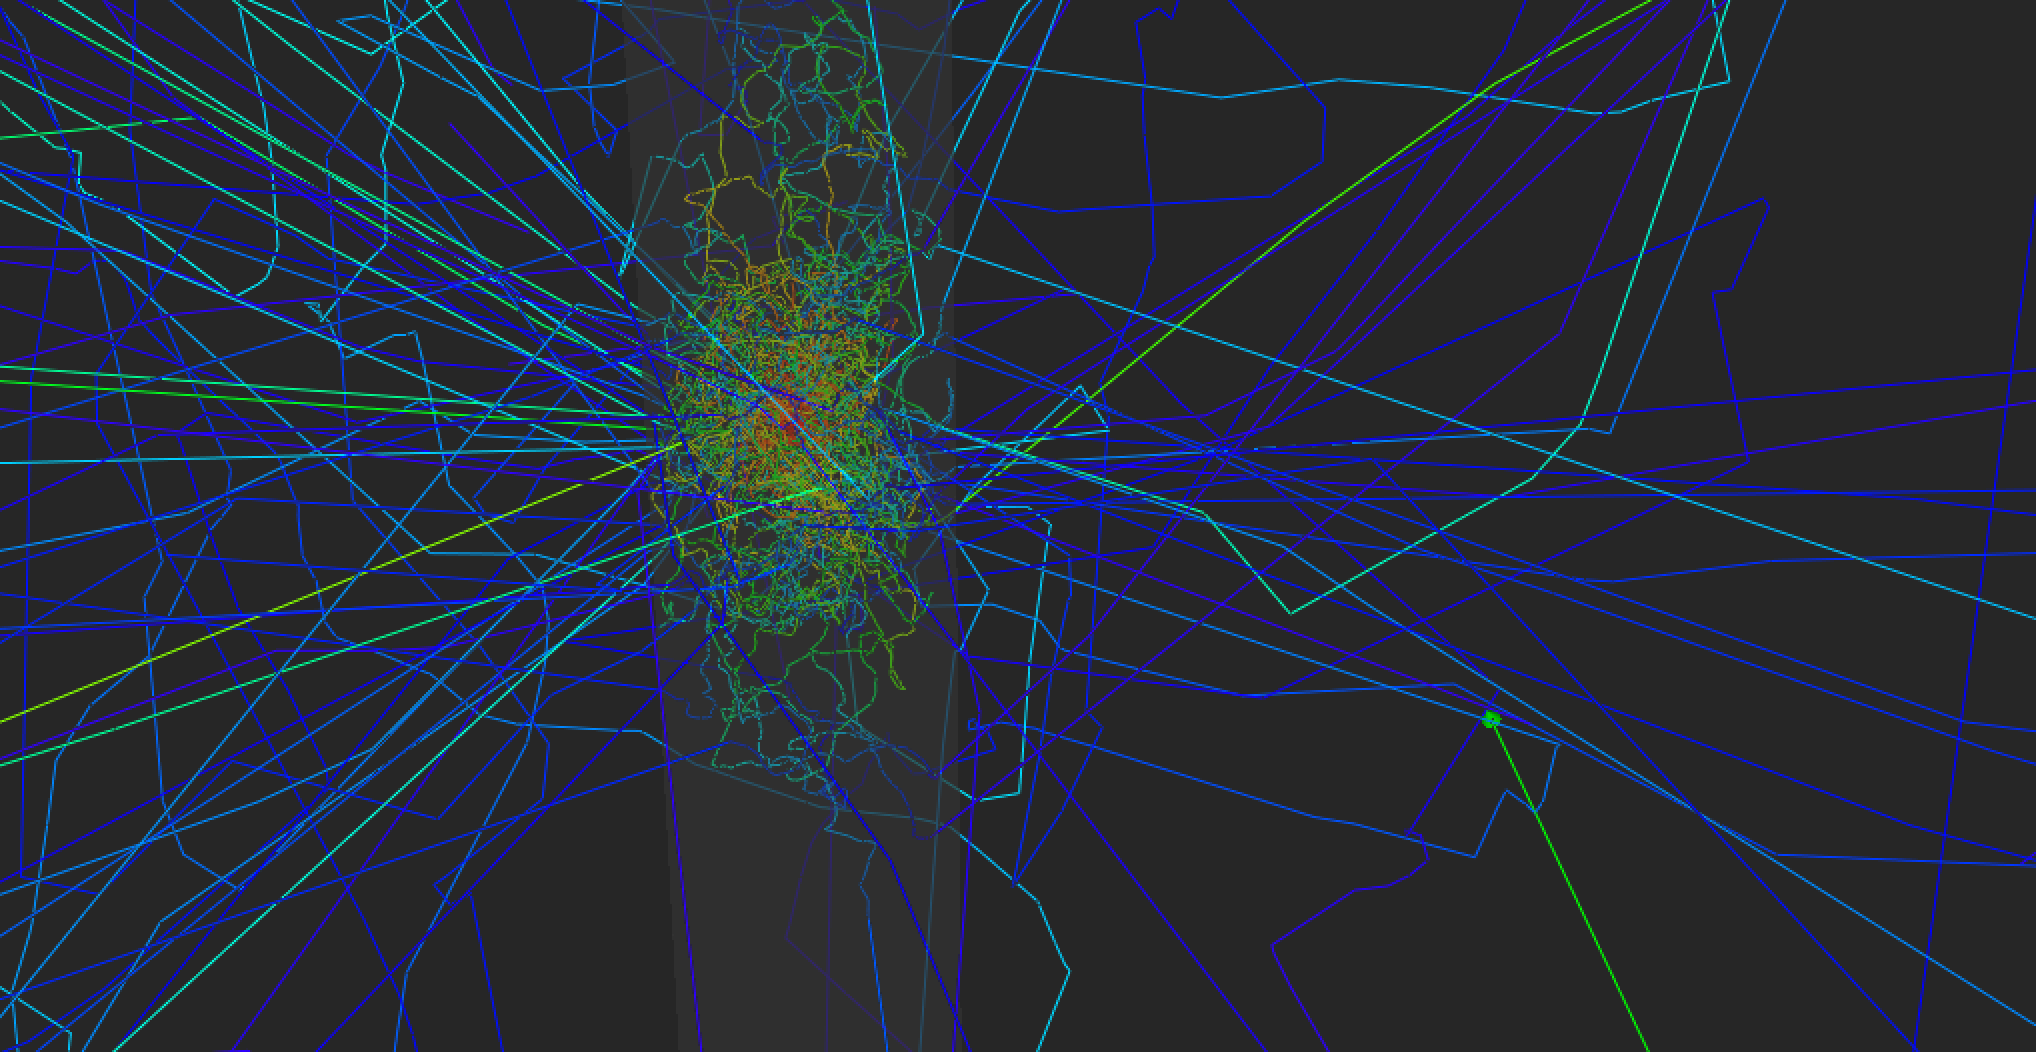
\includegraphics[width=.32\textwidth, trim={6cm 4cm 13cm 1.5cm}, clip]{img/instant-absorption-steamshovel-sahmoo8O-turned-off}}
  \caption{Visualizing an instant-absorption test where photons are started within two nested cylinders. The outer cylinder is configured for instant absorption. No photon can pass through the area between both cylinders unless the instant absorption is turned off.}
  \label{fig:sahmoo8O}
\end{figure}

\FloatBarrier\newpage
\subsubsection{Arrival-Time Distributions}
\label{sec:arrival_time}

One way to test the behavior of statistical properties of a sample of
photons is to plot the arrival-time distribution of photons traveling
from a central position to receiving optical modules around the starting
position. Figure \ref{fig:eipau6Ag} shows arrival-time distributions for
this scenario being carried out with a flasher experiment compared to
two simulations with different hole-ice configurations each.

\sourcepar{The source for the simulations and for creating these histograms can be found in \issue{91}.}

\begin{figure}[htbp]
  \subcaptionbox{Top view of the detector strings in this simulation. The photons are started at the middle optical module of string 63, and are received by the optical modules of the surrounding strings 70, 71, 64, 55, 54, and 62.}{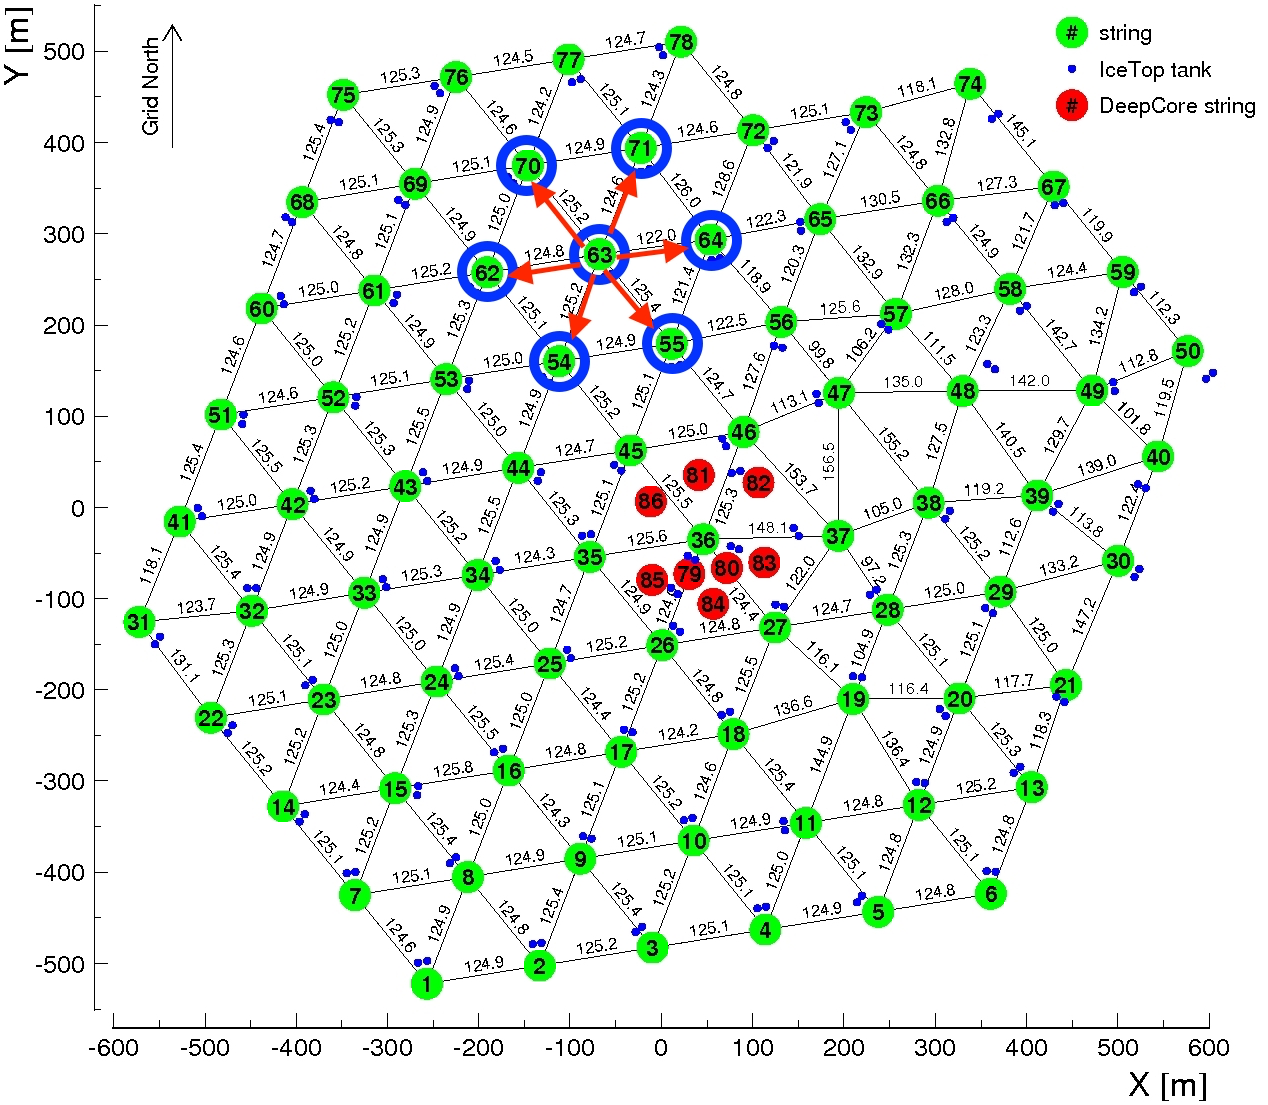
\includegraphics[width=.48\linewidth]{img/flasher-scenario}}
  \hfill
  \subcaptionbox{Photon-arrival-time distributions for different hole-ice configurations. The dashed lines indicate the mean arrival times.}{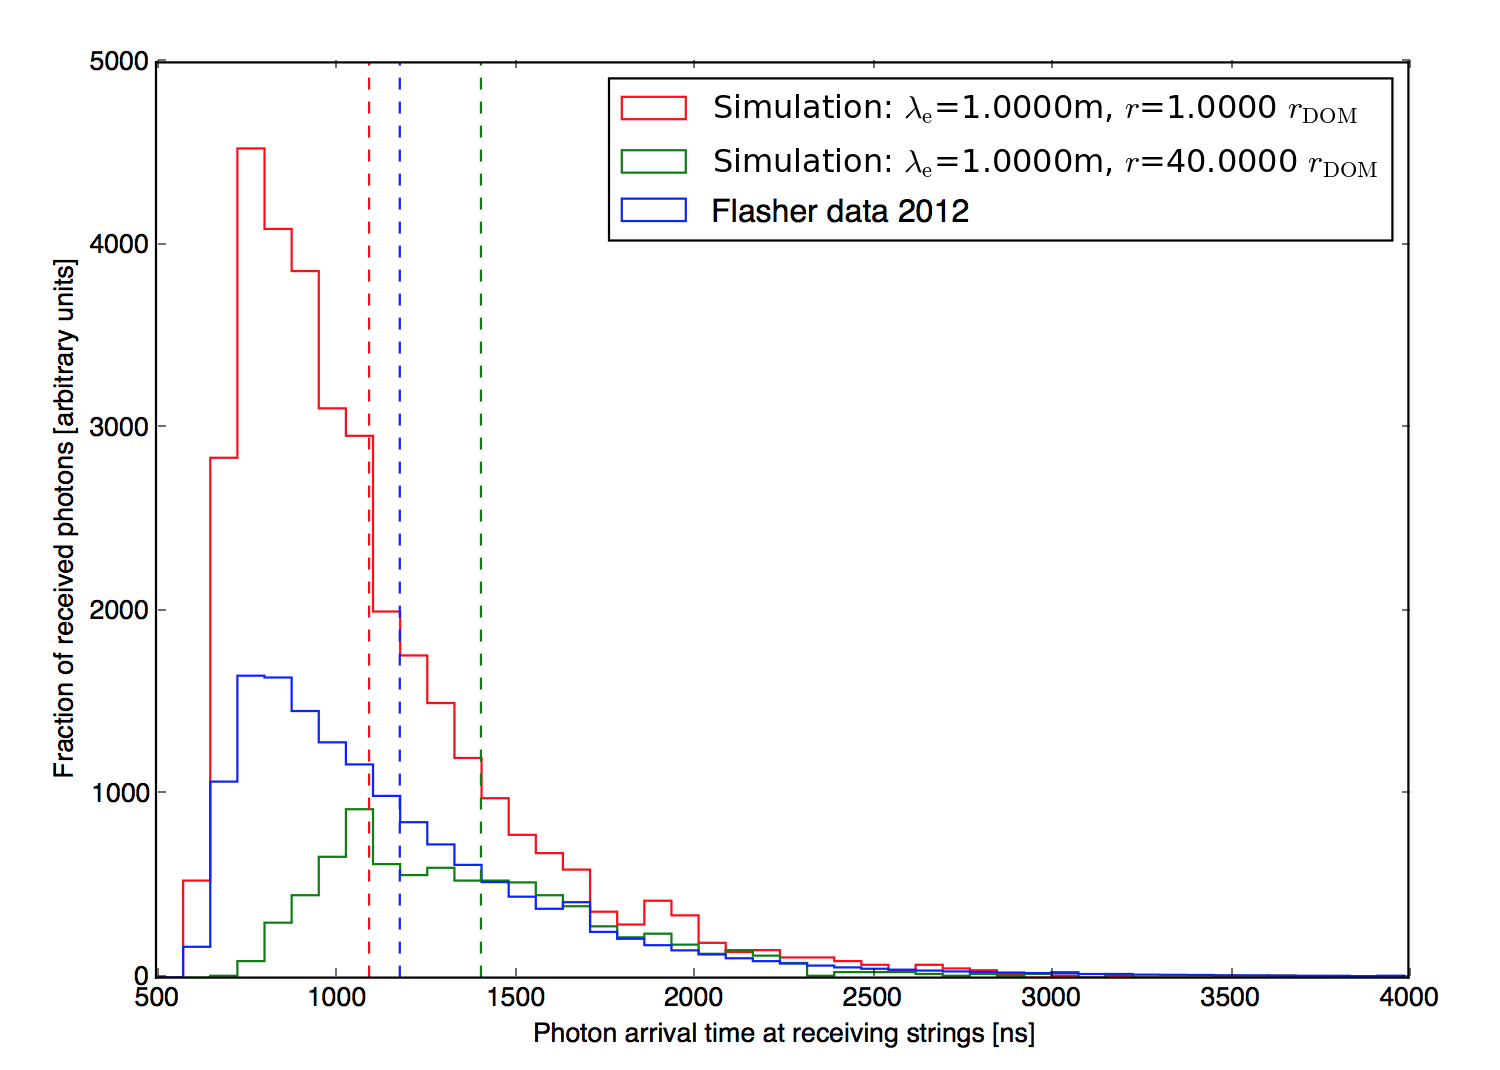
\includegraphics[width=.48\linewidth]{img/arrival-time-distribution-eipau6Ag}}
  \caption{Creating arrival-time distributions for photons propagating through hole ice. The photons are started at a central position and detected by optical modules around the starting position.}
  \label{fig:eipau6Ag}
\end{figure}

An estimation based on the mean scattering angle and the radius of the
hole-ice cylinder suggests that one would need a difference of the
hole-ice cylinder's radius of several meters to cause a difference in
the mean arrival time on the order of \(100\ns\). While this is no
realistic scenario as the drill hole's radius is only about \(50\cm\),
the simulation allows to use extreme scenarios to observe the effects
more noticeable.

From the comparison of the arrival-time distributions, note that the
distribution that is based on real data is comparable to the ones based
on simulations, which suggests that the new algorithm does not introduce
unexpected, unphysical effects to the photon propagation.

In the simulation where the hole-ice cylinders have a much larger
radius, the effects of the hole ice should be stronger. Indeed, the
comparison of the distributions shows three effects to expect from this
assumption: First, in the simulation with stronger hole-ice effect, less
photons arrive at the receiving optical modules in total as more photons
are scattered away by the hole ice. Secondly, for stronger hole ice, the
photons arrive later at the receiving optical modules, because they
spend more time scattering randomly within the hole-ice cylinder before
reaching the receiving optical module. Thirdly, for stronger hole ice,
the left-hand side of the distribution histogram is less steep, because
with more scattering points on the photon's path, there is a larger
number of possible paths, which leads to the arrival time being more
distributed.

While these effects confirm the expectations qualitatively, examining
other high-level observables allows to compare expectations to the
simulations' results even quantitatively. This is the subject of the
following sections, beginning with observing the photons' path-length
distributions.

\FloatBarrier\newpage
\subsubsection{Exponential Distribution of the Total Path Length}
\label{sec:total_path_length_distribution}

Let the \textbf{Total path length} of a photon be the summed distance
from the position where the photon is created, along the photon's path,
to the position where the photon is absorbed. The total path length
\(X\) of photons that propagate in a medium with an absorption
probability that is the same everywhere in the medium, for example
within a confined volume within the bulk ice, is expected to follow an
exponential distribution with a rate parameter corresponding to the
absorption probability, or equivalently the absorption length
\(\lambda\) within the
medium.\footnote{If the photons do not depend on each other, the number of photons that are absorbed at a certain path length does only depend on the absorption probability, or equivalently on the absorption length $\lambda$, and the number of photons remaining at this path length. When a photon is absorbed, the number of remaining photons decreases. Thus, the change in the number of photons is proportional to the number of photons, causing the number of photons absorbed at a certain path length following an exponential distribution. See also appendix \ref{sec:exponential_distribution}.}

\begin{equation}
  X: \ \ P(X \in [x; x + \dx[) \propto e^{\sfrac{-x}{\lambda}}, \ \ x \in \reals^+_0
\end{equation}

When propagating photons within a hole-ice cylinder, their path length
should also follow an exponential distribution, but with different
absorption length \(\lambda\hi\), as long as the absorption length is
sufficiently small such that most photons do not leave the cylinder
before being absorbed.

This behavior can be verified using a simulation. In the simulation, a
pencil beam of \(10^4\) photons is started within a hole-ice cylinder
with a radius of \(1.0\m\). The photons are started with a distance of
\(0.9\m\) to the cylinder center towards the cylinder center. Let the
effective scattering length within the cylinder be \(100.0\m\) and the
absorption length be \(0.1\m\). For each simulated photon, the total
path length is recorded.

\begin{figure}[htbp]
  %\smallerimage{cross-check-64-steamshovel}
  \caption{\steamshovel event display of the simulation of photons propagating and being absorbed within the hole-ice cylinder without medium transition. The photons are started within the hole-ice cylinder, which is represented by the grey cylinder, inwards. The detector module, which is represented by the white sphere in the center of the figure, is shown only to illustrate the size of the scenery and is configured not to interact with the simulated photons.}
\end{figure}

\sourcepar{The implementation of this cross check can be found in \issue{64}.}

The distribution of the total path length should follow an exponential
decay curve. From the rate of the decay, one should be able to read the
absorption length \(\lambda\) (see appendix
\ref{sec:exponential_distribution}).

\begin{figure}[htbp]
  \image{cross-check-64-exponential-distribution.png}
  \caption{Distribution of the total path length of simulated photons both started and absorbed within a hole-ice cylinder using the new medium-propagation algorithm. The distribution follows an exponential curve. The fitted absorption length is $\lambda_\text{abs}=0.1003\m \pm 0.0011\m$. The true absorption length used in the simulation is $0.1000\m$.}
  \label{fig:gieNa2Th}
\end{figure}

Indeed, the simulation yields the expected distribution of the total
path length (figure \ref{fig:gieNa2Th}). Via a curve fit, the absorption
length \(\lambdaabs\) can be determined for this simulation to be
\(\lambdaabs = 0.1003\m \pm 0.0011\m\), which is in accordance with the
true absorption length of \(0.1000\m\) used in the simulation.

\FloatBarrier\newpage
\subsubsection{Piecewise Exponential Distribution of the Total Path Length for One Medium Boundary}

This cross check aims to verify that the medium-boundary transition is
handled correctly when photons enter a hole-ice cylinder from outside.

In a simulation, a pencil beam of \(10^5\) photons is started in a
distance of \(2.0\m\) to cylinder center towards the hole-ice cylinder
with a radius of \(1.0\m\). The effective scattering length outside is
set to \(10^6\m\), inside to \(100\m\). The absorption length outside is
set to \(1.0\m\), inside to \(0.10\m\). As before, for each simulated
photon, the total path length, from the starting point of the photon
along the photon's trajectory to the point where the photon is absorbed,
is recorded.

\sourcepar{The implementation of this cross check can be found in \issue{65}.}

\begin{figure}[htbp]
  \smallerimage{cross-check-65-steamshovel}
  \caption{\steamshovel event display of the simulation of photons propagating through the hole-ice medium boundary. The photons are started outside and towards the hole-ice cylinder on the left hand side. As the scattering length within the cylinder is smaller, the photons scatter a lot more within the cylinder. The detector module is shown as a white sphere only to illustrate the size of the scenery and is configured not to interact with the simulated photons.}
\end{figure}

As the absorption lengths are different outside and inside the cylinder,
the histogram should now follow two separate exponential curves: The
left hand side of the histogram, which corresponds to the area outside
the cylinder, should follow an exponential curve governed by the
absorption length outside the cylinder. The right hand side, which
corresponds to the area within the cylinder, should follow an
exponential curve governed by the absorption length within the hole-ice
cylinder.

Note that the histogram's bins are proportional to the number
\(m(x):=\sfrac{-\d n(x)}{\dx}\) of photons that are absorbed within the
path length interval \([x; x+\dx[\), not the number \(n(x)\) of
remaining photons. Thus, the histogram is expected to show a jumping
discontinuity at the position of the medium
border.\footnote{See also appendix \ref{sec:exponential_distribution}.}

\begin{figure}[htbp]
  \image{cross-check-65-histogram}
  \caption{Distribution of the total path length of simulated photons started outside and absorbed within a hole-ice cylinder using the new medium-propagation algorithm. The distribution follows two exponential curves. The fitted absorption lengths are $\lambda_\text{abs,1} = 1.016\m \pm 0.310\m$ and $\lambda_\text{abs,2} = 0.101\m \pm 0.014\m$. The true absorption length in the simulation is set to $1.000\m$ outside, and to $0.100\m$ within the hole-ice cylinder.}
  \label{fig:iquo3Ou3}
\end{figure}

The simulation yields the expected distribution of the total path length
(figure \ref{fig:iquo3Ou3}). Via a curve fit, the absorption lengths
\(\lambda_\text{abs,1} = 1.016\m \pm 0.310\m\) and
\(\lambda_\text{abs,2} = 0.101\m \pm 0.014\m\) are in determined in
accordance with the true absorption length outside of \(1.000\m\) and
within the hole-ice cylinder of \(0.100\m\) set in the simulation.

\FloatBarrier\newpage
\subsubsection{Piecewise Exponential Distribution of the Total Path Length for Two Medium Boundaries}

This cross check aims to verify that the medium-boundary transition is
handled correctly when photons enter and leave a hole-ice cylinder.

In a simulation, a pencil beam of \(10^5\) photons is started in a
distance of \(1.5\m\) to the cylinder center towards the hole-ice
cylinder with a radius of \(0.5\m\). The effective scattering length
outside and inside is set to \(10^6\m\). The absorption length outside
is set to \(1.0\m\), inside to \(0.75\m\). As before, for each simulated
photon, the total path length is recorded.

\sourcepar{The implementation of this cross check can be found in \issue{66}.}

\begin{figure}[htbp]
  \smallerimage{cross-check-66-steamshovel}
  \caption{\steamshovel event display of the simulation of photons propagating through a hole-ice cylinder. As the scattering length is chosen to be very large, the photon path appears as a single line.  The photons are started outside the hole-ice cylinder on the left hand side. Some of them are absorbed before entering the cylinder, some within the cylinder and some after leaving the cylinder on the right hand side. The detector module is shown as a white sphere only to illustrate the size of the scenery and is configured not to interact with the simulated photons.}
\end{figure}

As the simulated photons may now cross two different medium boundaries,
the distribution of the path lengths should follow three exponential
curves: On the left hand side of the histogram, which corresponds to the
photons that are absorbed before entering the hole ice, the histogram
should follow an exponential curve governed by the absorption length
outside. In the middle, which corresponds to the photons that are
absorbed inside the cylinder, the histogram should follow an exponential
curve governed by the absorption length within the hole ice. On the
right hand side, which corresponds to the photons that are absorbed
after leaving the hole-ice cylinder, the histogram should follow an
exponential curve, again, governed by the absorption length outside the
cylinder.

\begin{figure}[htbp]
  \image{cross-check-66-histogram}
  \caption{Distribution of the total path length of simulated photons, which start outside the cylinder, and may be absorbed before, within or after passing the cylinder, using the new medium-propagation algorithm. The distribution follows three exponential curves. The fitted absorption lengths are $\lambda_\text{abs,1} = 1.02\m \pm 0.22\m$, $\lambda_\text{abs,2} = 0.68\m \pm 0.19\m$, and $\lambda_\text{abs,3} = 1.07\m \pm 0.23\m$. The true absorption length in the simulation is set to $1.00\m$ outside, and to $0.75\m$ within the hole-ice cylinder.}
  \label{fig:io9eiDee}
\end{figure}

The simulation yields the expected distribution of the total path length
(figure \ref{fig:io9eiDee}). The absorption lengths
\(\lambda_\text{abs,1} = 1.02\m \pm 0.22\m\),
\(\lambda_\text{abs,2} = 0.68\m \pm 0.19\m\) and
\(\lambda_\text{abs,3} = 1.07\m \pm 0.23\m\) determined via a curve fit
are in accordance with the true absorption length outside of \(1.00\m\)
and within the hole-ice cylinder of \(0.75\m\) set in the simulation.

\FloatBarrier
\subsubsection{Distance to Next Scattering Point in Relation to the Distance From the Hole-Ice Center}
\label{sec:cross_check_71}

The cross checks of the previous sections refer to the absorption
length. To examine the scattering-length behavior of the photons
simulated using the new media-propagation algorithm, this cross check
observes the distance to the next scattering point in relation to the
distance from the hole-ice center at each scattering point.

In a simulation, a plane wave of 100 photons is started towards a
hole-ice cylinder. Let the hole-ice radius be \(0.50\m\). The scattering
length within the hole-ice cylinder is \(0.06\m\), the scattering length
in the surrounding bulk ice is \(1.48\m\). For each scattering step, the
distance to the next scattering point and the current distance to the
center of the hole-ice cylinder are recorded.

\sourcepar{The implementation of this cross check can be found in \issue{71}.}

\begin{figure}[htbp]
  \smallerimage{cross-check-71-steamshovel}
  \caption{\steamshovel event display of a simulation of a plane wave of photons propagating towards a hole-ice cylinder. The scattering length within the hole-ice cylinder is different from the scattering length within the surrounding bulk ice.}
  \label{fig:An7ik8pu}
\end{figure}

As the distance to the next scattering point should be exponentially
distributed, governed by the scattering lengths within and without the
hole-ice cylinder, the distance to the next scattering point should
differ in the following three regions:

\begin{enumerate}
  \item Well within the hole-ice radius, the distance to the next scattering point should be in the range of the scattering length of the hole ice.
  \item Well outside the hole-ice radius, the distance to the next scattering point should be in the range of the scattering length of the surrounding bulk ice.
  \item In the vicinity of the hole-ice-cylinder radius, there should be some kind of transition due to the complex geometrical simulation.
\end{enumerate}

\begin{figure}[htbp]
  \centering
  \subcaptionbox{All data points}{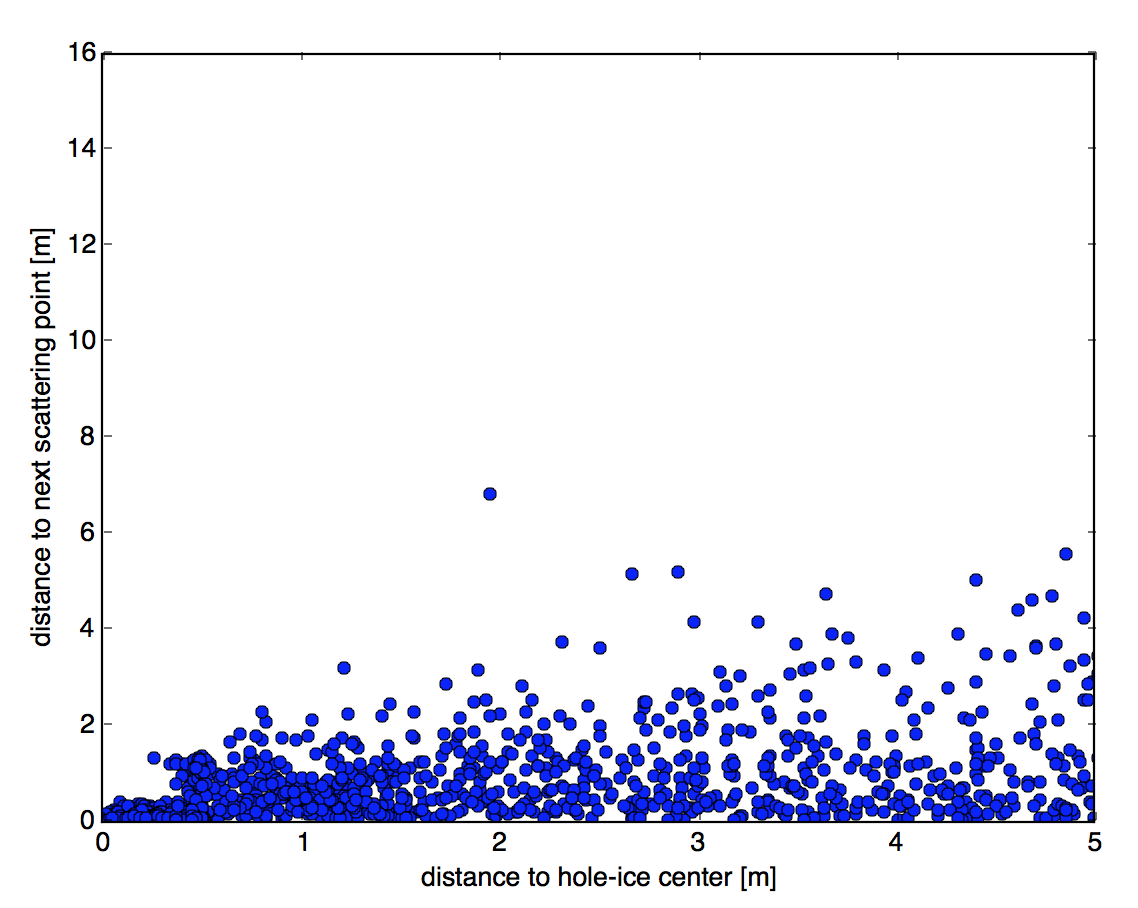
\includegraphics[width=0.48\linewidth]{img/cross-check-71-scatter}}\hfill
  \subcaptionbox{Averaged for bins of a width of  $10\cm$}{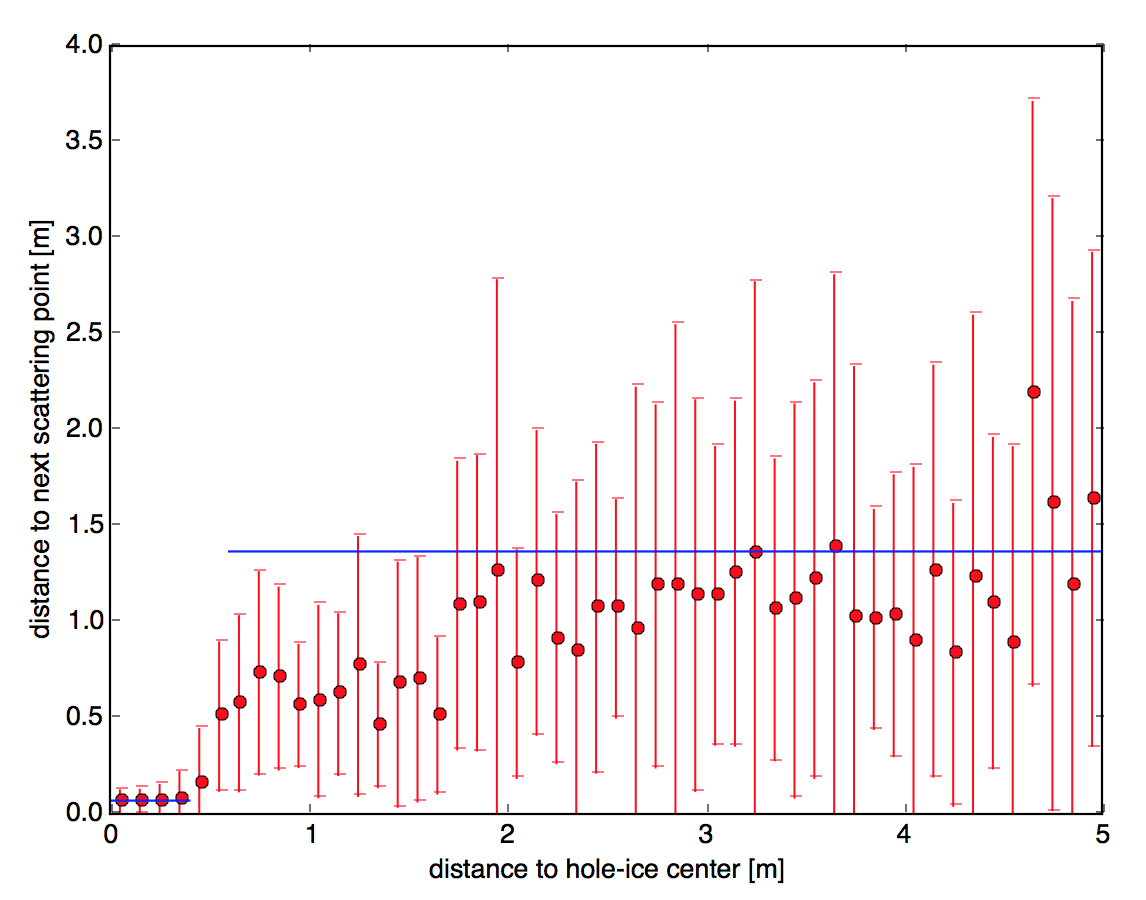
\includegraphics[width=0.48\linewidth]{img/cross-check-71-bins}}\hfill
  \subcaptionbox{Magnification of the vicinity of the hole-ice border}{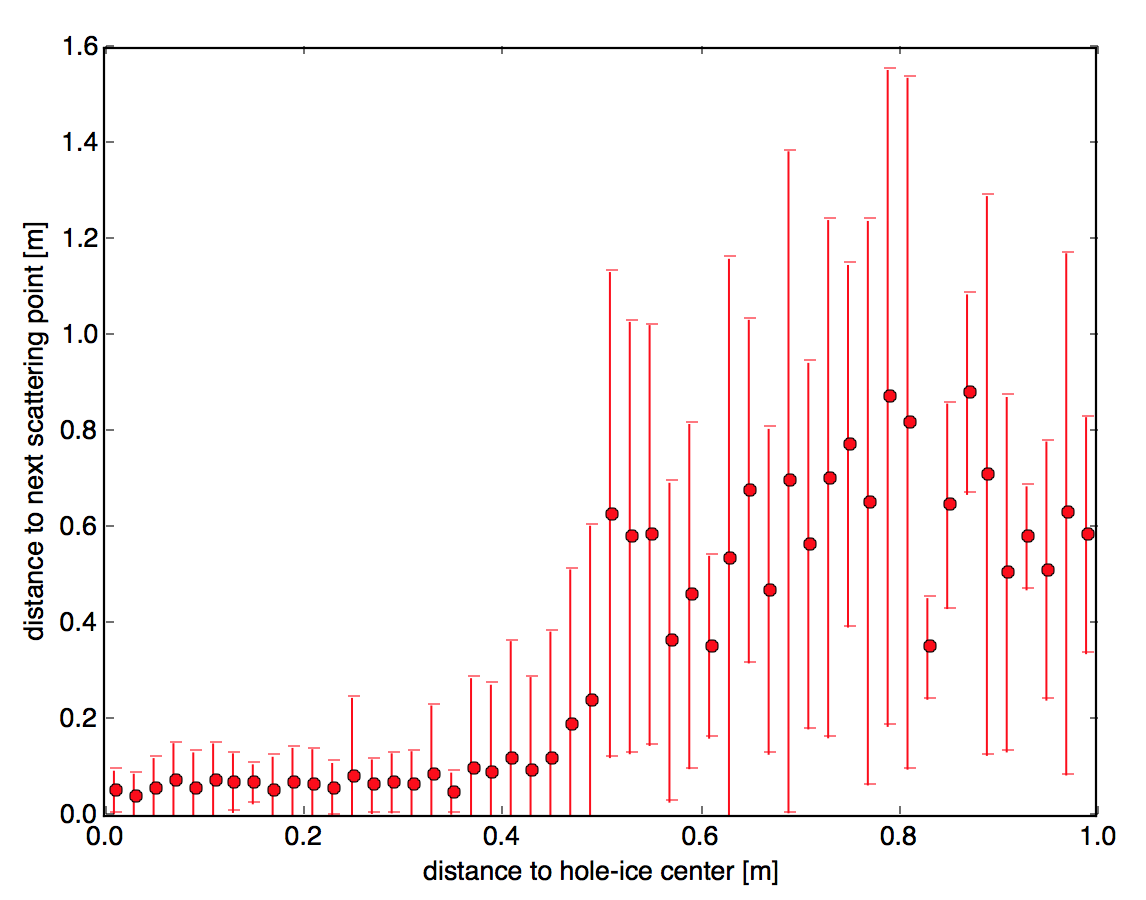
\includegraphics[width=0.48\linewidth]{img/cross-check-71-bins-vicinity}}
  \caption{For each scattering step of a simulation of photons entering a hole-ice cylinder, plot the distance to the next scattering step in relation to the current distance to the cylinder center. The mean distance to the next scattering point within $80\,\%$ of the hole-ice radius is fitted to $0.07\m \pm 0.07\m$. The mean distance to the next scattering point outside of $120\,\%$ of the hole-ice radius is fitted to $1.37\m\pm 1.37\m$. The true scattering length in the simulation is set to $0.06\m$ inside, and to $1.48\m$ outside the hole-ice cylinder.}
  \label{fig:eeYoid2p}
\end{figure}

Assuming an exponential distribution of the distance to the next
scattering point, the mean distance to the next scattering point within
\(80\,\%\) of the hole-ice radius is fitted to \(0.07\m \pm 0.07\m\),
the mean distance to the next scattering point outside of \(120\,\%\) of
the hole-ice radius is fitted to \(1.37\m\pm 1.37\m\) (figure
\ref{fig:eeYoid2p} b), which is in the range of the true scattering
lengths of \(0.06\m\) and \(1.48\m\) inside and outside the hole ice
respectively.

When plotting the local average of the distance to the next scattering
point for the vicinity of the hole-ice border (figure \ref{fig:eeYoid2p}
c), the curve shows no abrupt jump but a transition between both domains
as expected.
